
\section{23/01/2020 - first attempts with a 3D convolutional neural network}

\subsection{The dataset}
The dataset comprises 400 videos that have about 300 frames each; sometimes
299 - with 3 colors channels.
The resolution is 1920x1080. Sometimes transposed (vertical smartphone videos).

Even if the datapoints are effectively quite similar, they still require some operations
to make them have the same dimensionality. Moreover, the sheer size of the uncompressed
video suggests some preliminary scaling down of the input data.

\subsection{Tackling the huge dimensionality of the datapoints}

Every datapoint, loaded trough the library \texttt{skvideo}, has an uncompressed
size of 1.8 GB. In these conditions it seems an obvious choice to load one datapoint at once.
In order to have faster epochs, a slice of 15 frames is selected from each datapoint
scaling down the datapoint dimensionality to 93 MB.
The starting frame number of the frame slice will be chosen randomly. This will allow
all the frames of a video to be eventually considered trough all the epochs.

\subsection{Structure of the first model}

\begin{figure}[h]
\caption{First model: a 3d-convolutional neural network}
\centering
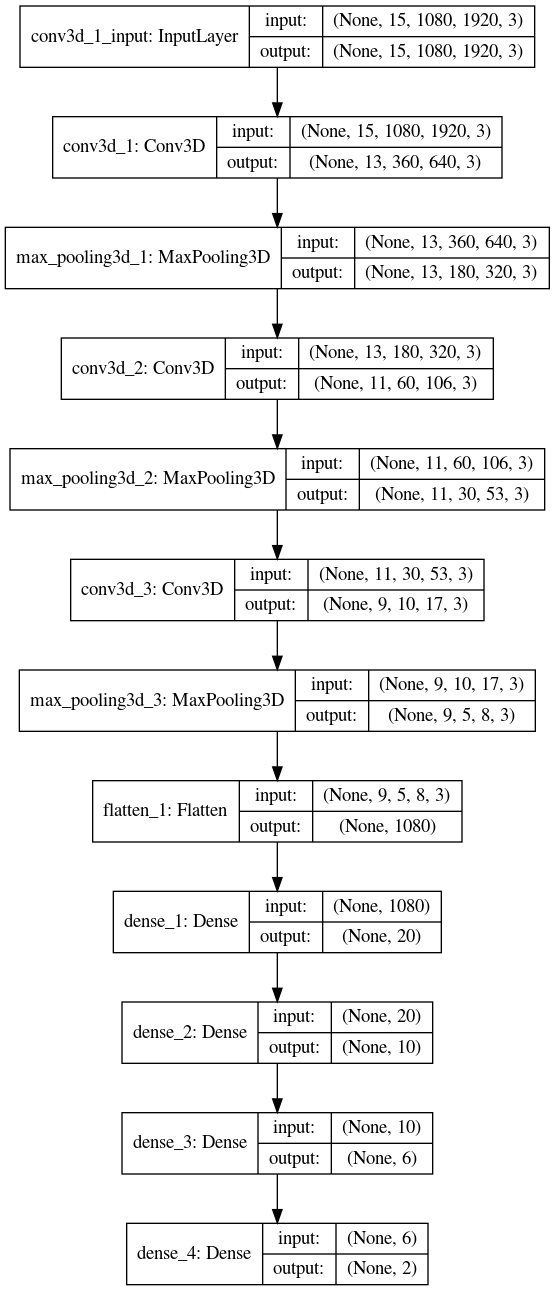
\includegraphics[width=0.5\textwidth]{first_model.png}
%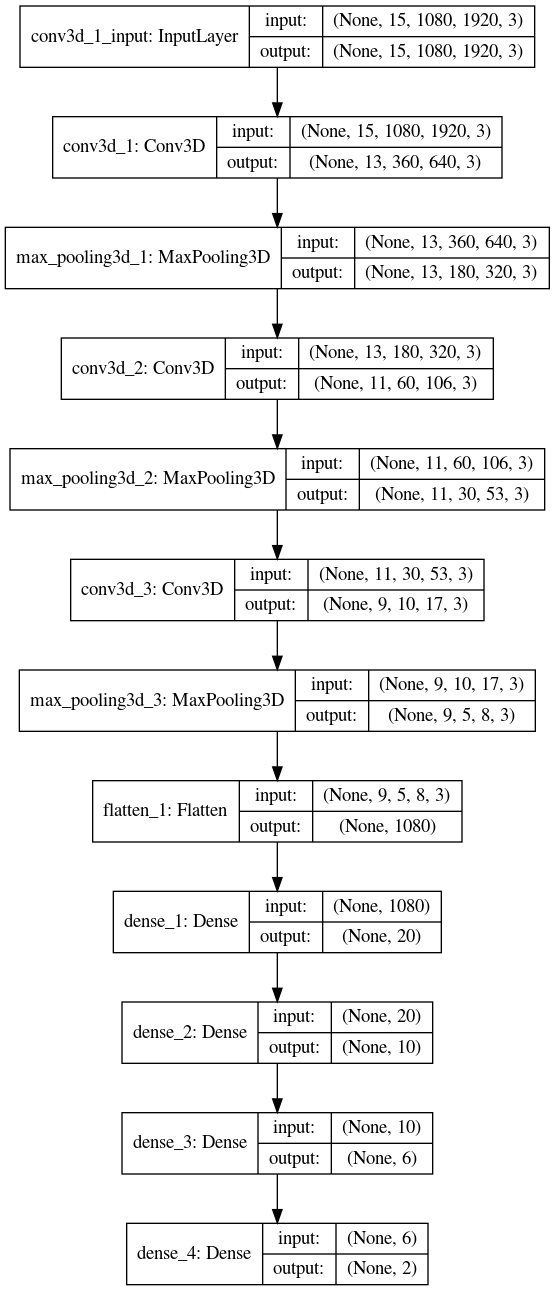
\includegraphics{first_model.png}
\end{figure}

The convolutional layers have been set with ELU activation functions.
The reason for this is to avoid dead units that emerge with ReLU activation functions
caused by 0 gradients.
For the dense layers the sigmoid activation function has been chosen.
Different activation functions could be also be investigated in the future,
such as ReLU and tanh, respectively for the convolutional and dense layers.
Also, not much tought has been given to regularization. But, since the network
seem to not fit on the training set, that's a problem for later.

The amount of parameters for this model is 22648.

\begin{figure}[h]
\caption{First model: parameter count for each layer}
\centering
\verbatiminput{first_model_summary.txt}
\end{figure}

\subsection{Considerations on using kernels that operate trough time}

What I noticed by watching the deepfake videos from the dataset is that some
of the videos were showing very scattered application of the face alteration.
Such abrupt changes are one of the first applications of convolutions for
image processing, such as edge detectors. Such characteristic would be 
detected here w.r.t. time.

For future reference, exclusively time-based convolution layers might be used
in a model - i.e. convolutional layers with kernel sizes that are 1 in both spatial
axes but arbitrary in the time dimension.

Also, factorized convolution could be used in a future model, as described in \cite{Burlacu}.

\subsection{Network output}

Since the output of the network is a 2-node softmax,
the first node is being used to learn a probability quantity of the input datapoint 
of being a deepfake. The second node, since it's softmax, will always output
1 minus the output of the first node.

The target vectors are hence $(1,0)$ for a deepfake and $(0,1)$ for a real video.

\subsection{Training}
Since training takes a considerable amount of time (about one hour for a training set
sweep), the number of training epochs is chosen to be as small as 100.
SGD has been chosen as optimization method. Adam/Nadam/Amsgrad/ND-Adam might be considered
as future improvement.

\subsection{Evaluation measures}

Currently two poorly-named (by myself) evaluation measures are being employed: unquantized average error,
and quantized average error.
Considering uniquely the value of the first output node, an unquantized error is the
difference between the expected value - 1 for deepfake, 0 for real - and the
emitted probability from the network. The unquantized average error
is simply the average value across the dataset.

The quantized error is, conversely, a rounding to the nearest integer of the unquantized error.
In a typical classification model a decision has to be made on how to use the output
of a neural network. Hence, the integer-rounding of the output represents the
decision on interpreting the binary classification model output either of one or the other category.
Hence, the quantized error is either 1 or 0 whenever that decision was correct or wrong.
The quantized average error is hence the average of the individual quantized errors
after a sweep of a validation/testing set.

In order to have a better overview on how the model is performing with regard to
the class unbalance problem, ratios of correct and wrong predictions disaggregated 
per class are being kept.

\subsection{Class unbalance problem}

The first model is not performing well. The output category is always the most frequent 
one, which is the deepfake videos, amounting to 323, while the real videos are only 77.
This class unbalance problem could be tackled by submitting more frequently
the real videos to the training. The ratio of fake/real is 4.2, hence one possible
future improvement could be to submit about 4 different slices of the real video to 
the fitting function for every slice of fake videos.

\subsection{Future improvements}
\begin{itemize}
\item localize the face and follow it to remove useless background
\item log number of parameters
\item log average loss
\item factorized convolutions
\item bottleneck layers
\item skip connections
\item different update methods
\item LSTMs/RNN
\item checkpoints to resume training
\end{itemize}
